%------------------------------------------------------------------------------
% Author(s):
% Varaun Ramgoolie
% Copyright:
%  Copyright (C) 2020 Brad Bachu, Arjun Mohammed, Varaun Ramgoolie, Nicholas Sammy
%
%  This file is part of Applied-Mathematics-Unit2 and is distributed under the
%  terms of the MIT License. See the LICENSE file for details.
%
%  Description:
%     Linear Programming graph for 2006 C q2
%------------------------------------------------------------------------------

\documentclass[crop,tikz]{standalone}
\usepackage{pgfplots}
\usepackage{../../../../src/tikzappmath}
\usetikzlibrary{patterns}

\begin{document}
	
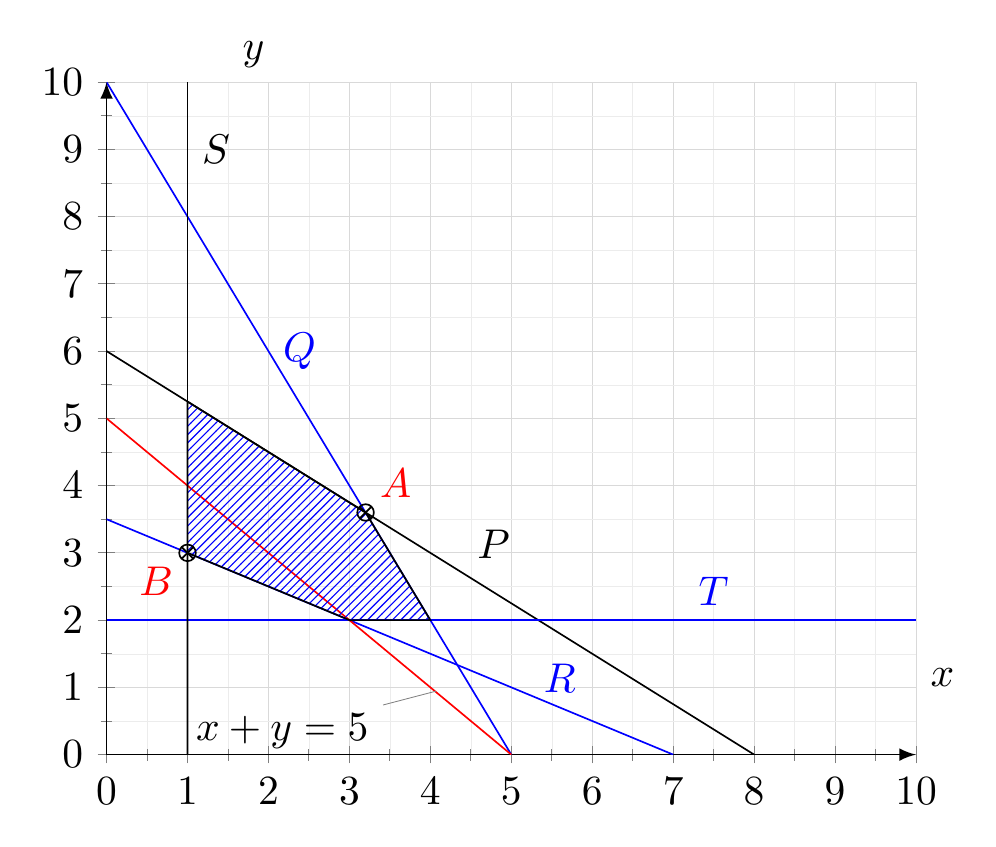
\begin{tikzpicture}[scale=1.5]
	\begin{axis}
		[
		xmin=-0,xmax=10,
		ymin=0,ymax=10,
		grid=both,
		grid style={line width=.1pt, draw=darkgray!10},
		major grid style={line width=.2pt,draw=darkgray!20},
		axis lines=left,
		minor tick num=1,
		enlargelimits={abs=0},
		axis line style={-latex},
		samples=100,
		domain = -20:20,
		ytick={0,1,...,10},
		xtick={0,1,...,10},
		xlabel={$x$},
		ylabel={$y$},
		x label style={at={(axis description cs:1,0.15)},anchor=north west},
		y label style={at={(axis description cs:0.15,1)},anchor=south west, rotate=-90}
		]
		
		\addplot [mark=dot,blue] coordinates{(5, 0)  (0,10)}	node[pos=0.6,blue, right] {$Q$};
		
		\addplot [mark=dot,blue] coordinates {(7,0) (0, 3.5)} node[pos=0.2,above,blue] {$R$};
		
		\addplot [mark=dot] coordinates {(8,0) (0, 6)} node[pos=0.45, above right] {$P$};
		
		\addplot [mark=dot] coordinates {(1,0) (1, 10)} node[pos=0.90, right] {$S$};
		
		\addplot [mark=dot, blue] coordinates {(0,2) (10, 2)} node[pos=0.75,above, blue] {$T$};
		
		\addplot [mark=dot, red] coordinates {(5,0) (0, 5)};
		
		\node [pin=190:{$x+y=5$}] at (axis cs:(4.25, 1) {};
		
		\addplot [pattern=north east lines,pattern color=blue] coordinates {(1,3) (3, 2) (4, 2) (3.2,3.6) (1, 5.25)} \closedcycle;	
		
		\addplot [mark=otimes] coordinates{(1, 3)} node[below left, red] {$B$};
		
		\addplot [mark=otimes] coordinates{(3.2, 3.6)} node[above right, red] {$A$};
		
	\end{axis}	
\end{tikzpicture}

\end{document}